\documentclass{article} % For LaTeX2e
\usepackage{nips15submit_e,times}
\usepackage{hyperref}
\usepackage{url}
%\documentstyle[nips14submit_09,times,art10]{article} % For LaTeX 2.09
\usepackage{amsmath}
\usepackage{graphicx}
\usepackage{subfig}
\title{Logistic and Softmax Regression for Handwritten Digits Classification}


\author{
Shilin Zhu \\
Ph.D. student, Computer Science\\
UCSD\\
La Jolla, CA \\
\texttt{shz338@eng.ucsd.edu} \\
\And
Yunhui Guo\\
Ph.D. student, Computer Science\\
UCSD\\
La Jolla, CA \\
\texttt{email} \\
}

% The \author macro works with any number of authors. There are two commands
% used to separate the names and addresses of multiple authors: \And and \AND.
%
% Using \And between authors leaves it to \LaTeX{} to determine where to break
% the lines. Using \AND forces a linebreak at that point. So, if \LaTeX{}
% puts 3 of 4 authors names on the first line, and the last on the second
% line, try using \AND instead of \And before the third author name.

\newcommand{\fix}{\marginpar{FIX}}
\newcommand{\new}{\marginpar{NEW}}

\nipsfinalcopy % Uncomment for camera-ready version

\begin{document}
\maketitle

\section{Logistic Regression via Gradient Descent}
\textbf{Derive the gradient for logistic regression:} \\
The cross-entropy cost function can be expressed as

\begin{equation}
	E(w) = - \sum_{n=1}^{N}[t^{n}\ln(y^{n})+(1-t^{n})\ln(1-y^{n})]
\end{equation}

where $t^{n}$ is the target label for example $n$ and $y^{n}$ is our prediction for this example. To perform gradient descent, we need to first compute the gradient (derivative) of the cost function with respect to the parameters. The gradient of cost function on example $n$ is

\begin{equation}
	-\frac{\partial E^{n}(w)}{\partial w_{j}} = \frac{\partial [t^{n}\ln(y^{n})+(1-t^{n})\ln(1-y^{n})]}{\partial w_{j}} 
\end{equation}

where $y^{n}$ is the prediction of logistic regression as

\begin{equation}
	y^{n} = g(\sum_{j=0}^{m}w_{j}x_{j}^{n})
\end{equation}

and $g(\cdot)$ is the sigmoid activation function and its derivative is

\begin{equation}
	g^{\prime}(z^{n}) = \frac{d(\frac{1}{1+e^{-z^{n}}})}{dz^{n}} = g(z^{n})(1-g(z^{n}))
\end{equation}

where $z ^{n}= \sum_{j=0}^{m}w_{j}x_{j}^{n}$. According to the chain rule in calculus, we can then compute the gradient (derivative) of the cost function on example $n$ with respect to the parameters as

\begin{equation}
	-\frac{\partial E^{n}(w)}{\partial w_{j}} = -\frac{\partial E^{n}(w)}{\partial y^{n}}\frac{\partial y^{n}}{\partial z^{n}}\frac{\partial z^{n}}{\partial w_{j}} = (\frac{t^{n}}{y^{n}}-\frac{1-t^{n}}{1-y^{n}})\cdot y^{n}(1-y^{n})\cdot x_{j}^{n} = (t^{n}-y^{n})x_{j}^{n}
\end{equation}

\textbf{Derive the gradient for regularized logistic regression:} \\

To prevent potential overfitting, regularization is used in logistic regression. The cross-entropy cost function with regularization term can be computed as

\begin{equation}
	E(w) = - \sum_{n=1}^{N}[t^{n}\ln(y^{n})+(1-t^{n})\ln(1-y^{n})] + \lambda * C(w)
\end{equation}

where $C(w)$ represents the complexity of the model. $L1$ and $L2$ regularizations are two most common functions people use

\begin{equation}
	C(w) = ||w||^{2} = \sum_{i, j}w_{i, j}^{2}(L2)
\end{equation}

\begin{equation}
	C(w) = |w| = \sum_{i, j}|w_{i, j}|(L1)
\end{equation}

Thus the gradient of cost function on example $n$ is 

\[
    -\frac{\partial E^{n}(w)}{\partial w_{j}} = 
\begin{cases}
    (t^{n}-y^{n})x_{j}^{n} - 2\lambda w_{j},& \text{if } L2\\
    (t^{n}-y^{n})x_{j}^{n} - \lambda sign(w_{j}), & \text{if } L1
\end{cases}
\]

Note that we can always add a factor of $1/N$ to scale the cost and gradient to somehow speed up the learning, and this will not change the optimization results (learned parameters).


\section{Softmax Regression via Gradient Descent}
\subsection{Problem definition}
In this problem, we need to classify MNIST datasets using softmax regression. In the experiments, we only use the first 20,000 training images and the last 2,000 test images.

\subsection{Methods}
\textbf{Derive the gradient for Softmax Regression:} \\
The cross-entropy cost function can be expressed as,

\begin{equation}
	E = - \sum_{n}\sum_{k=1}^{c}t_k^n\ln y_k^n
\end{equation}

Where, 
\begin{equation}
	y_k^n = \frac{\exp{(a_k^n)}}{ \sum_{k'}\exp{(a_{k'}^n})}
\end{equation}
And, 
\begin{equation}
	a_k^n = w_k^Tx^n
\end{equation}
We can calculate the gradient for softmax regression as follows,
\begin{equation}
\begin{split}
-\frac{\partial E^n(w)}{\partial w_{jk}}& = - \frac{\partial E^n(w)}{\partial a_k^n}\frac{\partial a_k^n}{\partial w_{jk}} \\
& = -\sum_{k'} \frac{\partial E^n(w)}{\partial y^n_{k'}} \frac{\partial y^n_{k'}}{\partial a^n_k}\frac{\partial a_k^n}{\partial w_{jk}} \\
\end{split}
\end{equation}
And 
\begin{equation}
\begin{split}
\frac{\partial y^n_{k'}}{\partial a^n_k} =  y^n_{k'}\delta_{kk'} - y_{k
'}y_{k}\\
\end{split}
\end{equation}
Where $\delta_{kk} = 1$ if $k = k'$, otherwise $\delta_{kk} = 0$.
And
\begin{equation}
\begin{split}
	\frac{\partial E^n(w)}{\partial y^n_{k'}} = -\frac{t_{k'}}{y_{k'}}
\end{split}
\end{equation}
Substitute Equation (5) and Equation (6) into Equation (4) we get,
\begin{equation}
\begin{split}
	-\frac{\partial E^n(w)}{\partial w_{jk}} = (t_k - y_k)x_j^n 
\end{split}
\end{equation}

\textbf{Derive the gradient for Softmax Regression with Regularizations:} \\

With regularization, generally the loss function can be writen as,
\begin{equation}
J(w) = E(w) + \lambda C(w)
\end{equation}
If we use $L_1$ regularization in softmax regression,
\begin{equation}
	\lambda C(w) = \lambda C_{L_1}(w) =   \lambda \sum_{ij}|w_{i,j}|
\end{equation}

We can compute the derivate of $\frac{\partial C}{\partial w}$ as follows,
\begin{equation}
	\frac{\partial C_{L_1}(w)}{\partial w_{ij}} = sign(w_{i,j})
\end{equation}
Where $sign(x) = 1$ if $x > 0$, $sign(x) = 0$ if $x = 0$ and $sign(x) = -1$ if $x < 0$.

If we use $L_2$ regularization in softmax regression,

\begin{equation}
\lambda C(w) = \lambda C_{L_2}(w) =   \lambda \sum_{ij}w_{i,j}^2
\end{equation}

We can compute the derivate of $\frac{\partial C}{\partial w}$ as follows,

\begin{equation}
\frac{\partial C_{L_2}(w)}{\partial w_{ij}} = 2w_{i,j}
\end{equation}

In summary, 
  \[
-\frac{\partial J^n(w)}{\partial w_{j,k}} =\left\{
\begin{array}{ll}
(t_k - y_k)x_j^n - \lambda sign(w_{j,k}),\qquad \text{if use $L_1$ regularization} \\
(t_k - y_k)x_j^n - 2\lambda w_{j,k}, \qquad \text{if use $L_2$ regularization}
\end{array}
\right.
\]
\\

\textbf{Preprossing}: First, we extract the first 20,000 training images and the last 2,000 test images. Then normailize the images to make sure the pixel values are in the range of [0,1]. Convert the labels to one-hot vectors. Divide the training images into two parts, the first 10\% are used for as a hold-out set and the rest 90\% are used for training.
\\

\textbf{Experiments settings:} We use standard normal distributions to initilize the weights. We use an initial learning rate $\eta({0})$ = 0.004 and use equation $\eta({t}) = \eta{(0)}/(1+t/T)$ to anneal the learning rate by reducing it over time. $t$ is used to index the epoch number and $T$ is a metaparameter which is set to be 2. In the
experiements, we find that above learning settings work best.   \\
To determine the best type of regurization and the best $\lambda$, we try $L_2$ regularization and $L_1$ regularization seperately. For the $L_2$ regularizartion, we search the best $\lambda$ in the set $\{0.01, 0.001, 0.0001\}$. If the accuracy on the hold-out set decreases for 3 epochs, we stop the algorithm and use the weights with the highest accuracy on the hold-out set as the final answer. For the $L_1$ regularization, we follow the same steps. We run the 1000 epochs for each setting. \textbf{}Then we compare the results got from these two regularization methods and use the best one as the final result.
 
\subsection{Results}
(a) In the experiments, we find that using $L_2$ regularization with $\lambda = 0.01$ obtain the best result on the validation set with an accuracy of 0.9045\% on the validation set. The accuracy is 0.927\% on the test set under such settings. \\

To further examine the performance of the algorithm, we try other $\lambda$s. We choose $\lambda$ in the set $\{0.05,0.005,0.0005\}$ and use $L_2$ regularization. The highest accuracy on the validation set is $0.8965\%$ with $\lambda = 0.0005$. And the test accuracy is $0.933\%$ which is slightly higher than when $\lambda = 0.01$. So in following experiments, we fix $\lambda$ to be 0.0005.

\begin{figure}[t]%
	\centering
	\subfloat[The percent correct over the number of training iterations for the training, hold-out and test set.]{{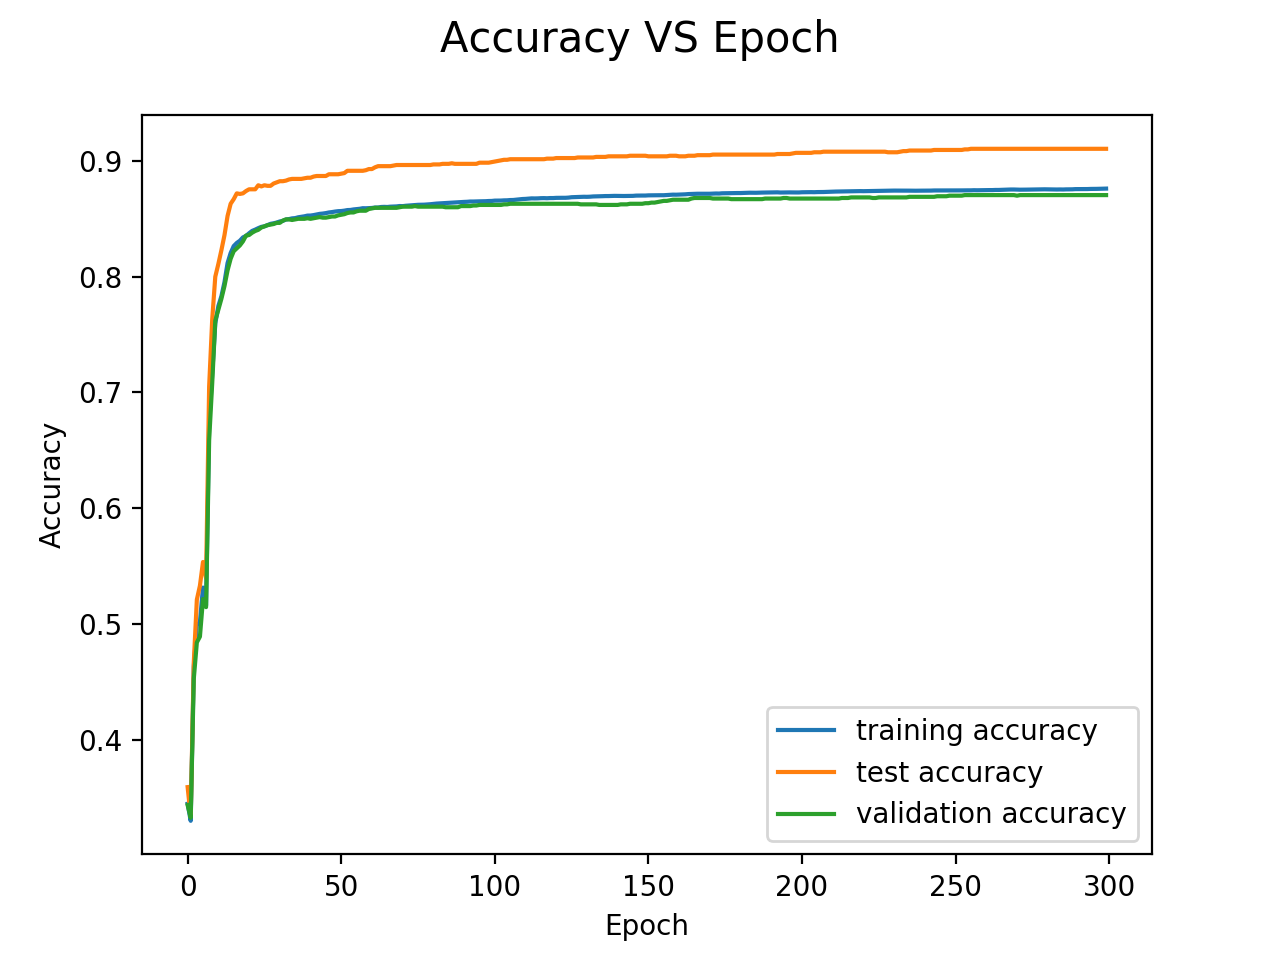
\includegraphics[width=1.8in,height=1.8in]{../softmax/figs/accuracy.png} }
		\label{fig: 1}
	}%
	\qquad
	\subfloat[The value of the loss function over the number of training iterations for the training, hold-out, and test set.]{{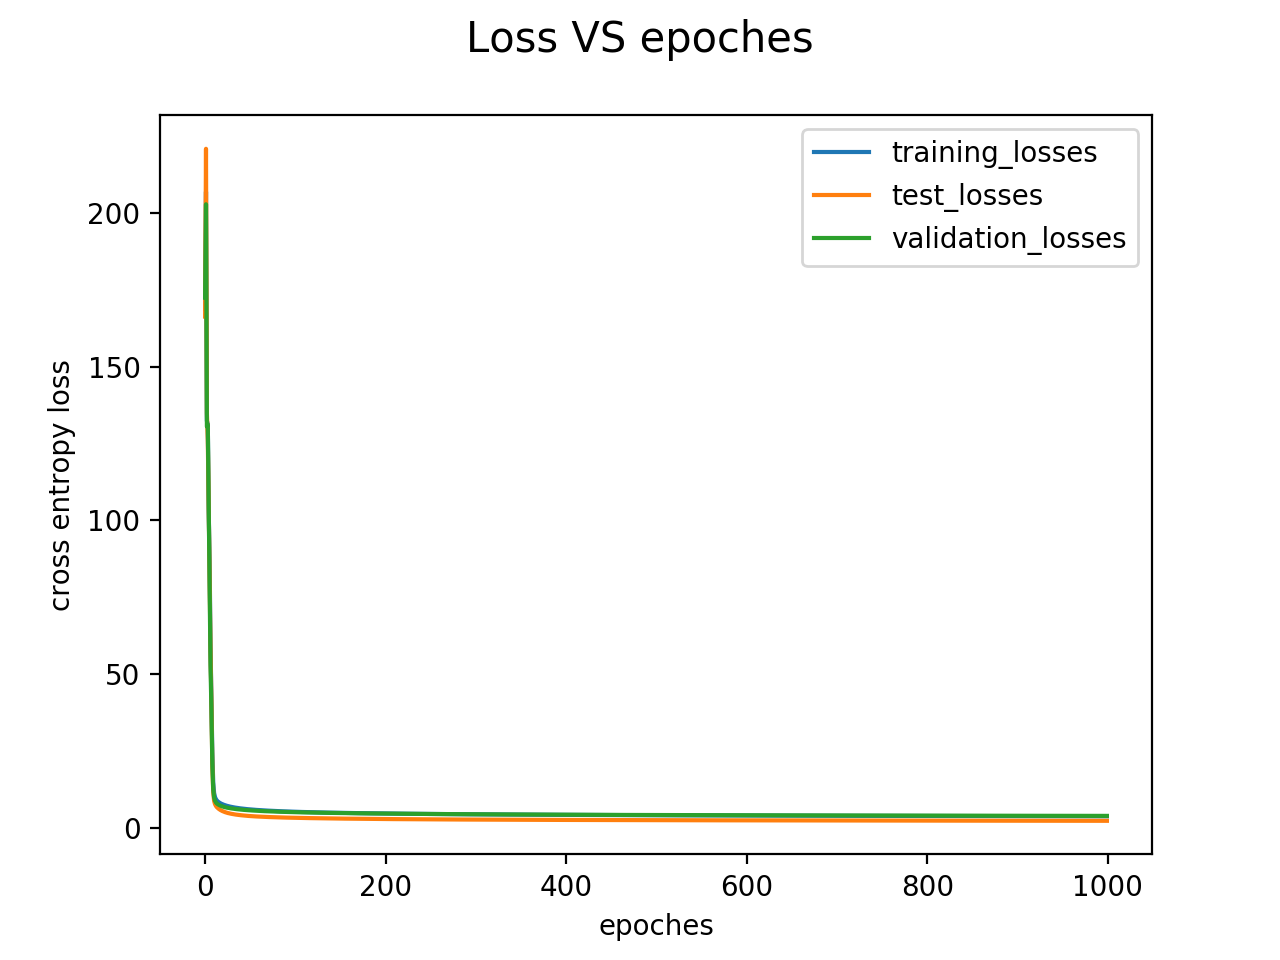
\includegraphics[width=1.8in,height=1.8in]{../softmax/figs/loss.png}  }
			\label{fig: 2}%
		}%
	\caption{The performance of the algorithm over the number of training iterations. }%
\end{figure}

\begin{figure}[t]
	\centering	
	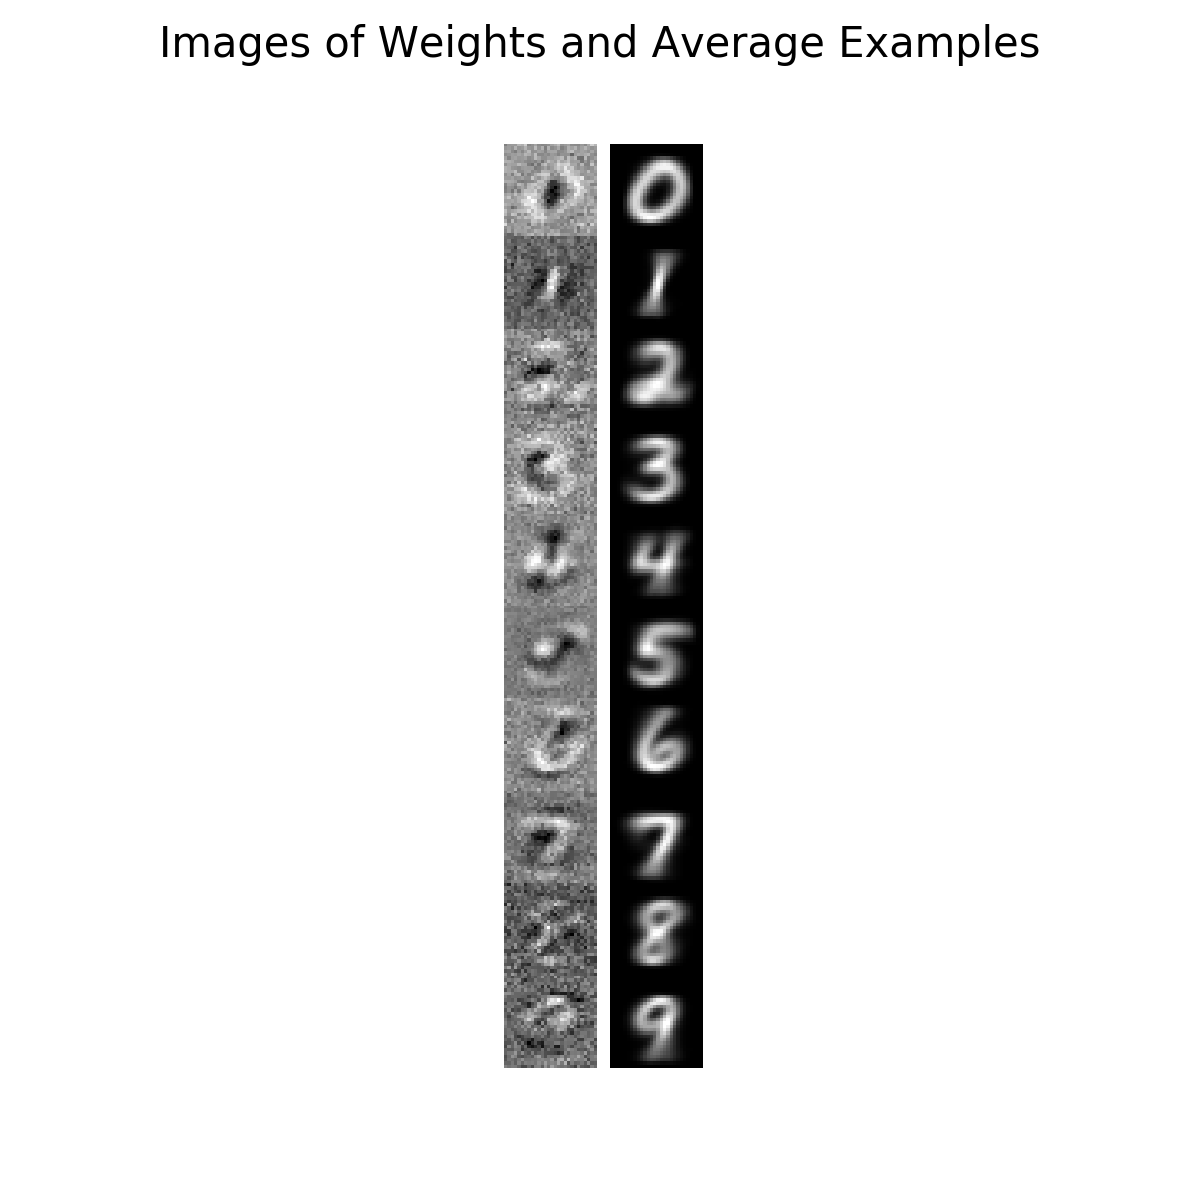
\includegraphics[width=2.7in,height=1.2in]{../softmax/figs/image_of_weights_and_digits.png} 
	\caption{Images of the weights and the average examples.}
	\label{fig: 3}
\end{figure}

(b) In this experiement, we use $L_2$ regularization with $\lambda = 0.005$. The figure is shown in Fig \ref{fig: 1}.


(c) In this experiement, we use $L_2$ regularization with $\lambda = 0.005$. The figure is shown in Fig \ref{fig: 2}. Note that we use the sum of loss of individual data rather than the average one.

(d) We plot the results in Fig \ref{fig: 3}. 



\subsection{Discussion}
From \ref{fig: 1} and \ref{fig: 2} we can see that the loss function went up before going down. And the accuracy and loss function converges quickly and then becomes smooth. The plausible reason is that the learining rates in the first few epoches maybe a little large but after "annealing", the learning rates are suitable enough to make the algorithm converge. Setting the learning rate too small initially may let the algorihtm too slow to converge or just being stucked. And we also see that there is no overfitting occurs. One possible reason for this is that the impact of the regularization. Another one is that the algorithm correctly learns the pattern underlying the data at hand.

From \ref{fig: 3} we can see that the image of the weight and the corresponding image of the average digit is almost the same. The reason is that we classify the images based on the inner product of the pixels with the weights. And the inner product is maximized when the angle between the weight and the image is zero. So we see that the image of the weight and the corresponding image of the average digit is similar.

\subsubsection*{Acknowledgments}

. 

\subsubsection*{References}

\end{document}
